\section{Experiments}
\label{sec:experiments}

Our evaluation addresses five questions: at fixed memory, how many invalid expensive point queries each admission index forwards (RQ1); how much learned region-wise AMQ allocation helps beyond global or handcrafted partitions (RQ2); how robust that benefit is under train/test shift, replay, and occupancy pressure (RQ3); how admission decisions translate into backend queueing and worker provisioning (RQ4); and whether public trace-conditioned arrival/account skew changes the conclusions (RQ5).

\subsection{Experimental Setup}

\begin{table}[t]
  \centering
  \footnotesize
  \caption{Backend verifier latency.}
  \label{tab:backend-benchmark}
  \begin{tabularx}{\columnwidth}{lXX}
    \toprule
    Metric & Argon2id & PBKDF2 \\
    \midrule
    Parameters
      & \(t=3\), \(m=65536\) KiB, \(p=1\)
      & iter.\(=600000\), hash\(=\texttt{SHA-256}\), dkLen\(=32\) B \\
    Verifier calls
      & 78,620
      & 78,620 \\
    Mean
      & 122.07 ms
      & 184.32 ms \\
    Median (P50)
      & 99.71 ms
      & 177.76 ms \\
    P95
      & 155.88 ms
      & 192.04 ms \\
    P99
      & 162.96 ms
      & 316.78 ms \\
    Single-worker cap.
      & 8.19 verif./s
      & 5.43 verif./s \\
    \bottomrule
  \end{tabularx}
\end{table}

\begin{table}[t]
\centering
\scriptsize
\setlength{\tabcolsep}{3pt}
\caption{Benign and attack workload model.}
\label{tab:workload-model}
\begin{tabular}{p{0.24\linewidth} p{0.66\linewidth}}
\toprule
\textbf{Item} & \textbf{Specification} \\
\midrule
\multicolumn{2}{l}{\textit{Benign workload}} \\
Horizon & 7 days \\
Session count & Poisson with bucket-specific \(\lambda\), scaled by weekday/weekend factors \\
Rate bucket & rare / weekly / daily / power \\
Session pattern & success / typo-success / old-password-success / new-device-success / benign-failure / repeat-success \\
Time & hourly weights: morning / afternoon / evening / night / mixed \\
Region & mostly home; occasional adjacent/far travel \\
Device & known-device pool; occasional new device \\
\midrule
\multicolumn{2}{l}{\textit{Attack workload}} \\
Credential stuffing & existing accounts; leaked current/old/wrong pairs; far region, attacker UA \\
Password spraying & broad accounts; top-\(k\) passwords; distributed attacker IPs \\
Brute force & small target set; repeated guesses; short bursts \\
Old-password replay & password-changed accounts; old password only; attacker-controlled metadata \\
Adaptive evasion & sampled accounts; mixed guesses; benign-like UA/device/region \\
Benign-mimic flood & broad high-volume accounts; mostly wrong guesses; benign-like metadata \\
Nonexistent-account flood & fake/mixed accounts; random/common guesses; mixed benign-like/attacker-like metadata \\
Low-and-slow distributed & many accounts; sparse guesses; wide IP pool, benign-like timing \\
Timing probe & repeated target variants; incorrect probes; metadata permutations \\
\bottomrule
\end{tabular}
\end{table}

\begin{table}[t]
\centering
\caption{Baselines and metrics.}
\footnotesize
\setlength{\tabcolsep}{2.5pt}
\renewcommand{\arraystretch}{0.94}
\begin{tabularx}{\columnwidth}{@{}p{0.82cm}p{1.95cm}X@{}}
\toprule
Type & Item & Description \\
\midrule
\multicolumn{3}{@{}l}{\textit{Baselines}} \\
Ext. & Backend only & No pre-screening; forwards all requests. \\
Ext. & Rate limit & Progressive throttling or lockout after failures~\cite{nist_sp800_63b_4_2025,owasp_authentication_cheat_sheet}. \\
Ext. & Blocklist & Registration-time or policy-side weak-password denylist screening~\cite{nist_sp800_63b_2017,nist_sp800_63b_4_2025,owasp_authentication_cheat_sheet}. \\
Ext. & Global Bloom & Single global Bloom filter over the same PRF trapdoors and total memory budget as TRAPS~\cite{Bloom1970BloomFilter,broder2004network}. \\
Diag. & Peppered tag & Exact keyed fast-verifier tag with uniform or adaptive tag lengths. \\
Diag. & Hash partition & Non-learned partitioned Bloom filter using hash/account partitions under the same total memory. \\
Diag. & Risk partition & Handcrafted-risk partition using known-password markers without a learned router. \\
Diag. & Neg. cache & Exact account-local cache of backend-confirmed invalid tuples. \\
Diag. & Oracle AMQ & Non-deployable allocation using held-out invalid-query masses. \\
Op. & Rate+tag & Token-bucket throttling plus peppered tags; may throttle valid requests. \\
Int. & TRAPS-Single & Risk-partitioned single-layer AMQ screening. \\
Int. & TRAPS-Layered & Risk-partitioned layered screening with early negative exits. \\
Int. & TRAPS-Strict & Stricter capped allocation policy; no login-time risk-only rejection. \\
\midrule
\multicolumn{3}{@{}l}{\textit{Metrics}} \\
Pri. & Valid-cred. FNR & Valid credentials rejected in error. \\
Pri. & Invalid fwd. rate & Invalid requests sent to the backend. \\
Pri. & Backend checks & Number of backend password verifications. \\
Aux. & Load reduction & Derived reduction in backend workload relative to no pre-screening. \\
Pri. & Login p95 latency & 95th-percentile latency of legitimate logins~\cite{dean2013tail}. \\
Aux. & Frontend mean cost & Mean compute cost of frontend screening. \\
Aux. & Memory footprint & Memory used by the screening layer. \\
Aux. & Backend time & Total backend verification time. \\
Aux. & Capture rate & Invalid requests blocked; complement of invalid forwarding rate. \\
\bottomrule
\end{tabularx}
\label{tab:baseline_metric_compact}
\end{table}

\paragraph{Configurations}
Experiments run on 64-bit Microsoft Windows~11 Pro 24H2 with a 13th Gen Intel Core i9-13900KF CPU and 16\,GB RAM. The Python~3.12 prototype uses optimized OpenSSL and Argon2 library backends, and all baselines and TRAPS variants share the same Argon2 and PBKDF2 parameters. Timing microbenchmarks use the Windows high-performance power plan and synchronous single-worker execution to calibrate per-attempt verifier cost, not production throughput. The reproducibility package\footnote{Anonymous artifact URL: \url{https://anonymous.4open.science/r/ICDETRAPS20260609}.} includes the workload generator, replay scripts, plotting scripts, and exported audit denominators.

\paragraph{Measurement modes}
We use five modes: a verifier-path benchmark for single-worker backend cost; replay evaluation over identical event streams; seeded production-baseline frontiers with denominators and confidence intervals; distribution-shift grids over target skew, risk drift, replay, and occupancy pressure; and method-specific bounded-worker queueing using the measured Argon2 service time.

\paragraph{Prototype and evaluation pipeline}
All methods share the same \texttt{verify\_password} interface and backend registry format; TRAPS changes only which attempts are forwarded. Each forwarded attempt therefore incurs the same backend path, including registry lookup, stored-hash parsing, salt and parameter recovery, password hashing, and constant-time comparison. Passwords are drawn from the \texttt{current\_password} field of \texttt{accounts.csv}, preserving the password-length distribution, and verification reads the complete stored hash from \texttt{backend\_registry.csv}. We calibrate forwarded-attempt cost with 78{,}620 single-worker verifier calls per backend configuration; the benchmark excludes network I/O, client load generation, queueing, frontend screening, and inter-request concurrency.

For auxiliary backend-work accounting, if a method forwards \(F\) attempts and the measured mean verifier cost is \(\bar{t}_{\mathrm{verify}}\), we compute
\[
W_{\mathrm{verify}} = F \cdot \bar{t}_{\mathrm{verify}} .
\]
Main method comparisons are based on forwarded attempts under the shared backend path; the benchmark only maps those attempts to an implementation-level cost scale.

\paragraph{Data preparation and label construction}
Credential-match inference is allowed only when credential evidence is user-unique or an explicit event-level validity label is present; otherwise, the match label remains unknown. A valid attempt is a labeled match to a represented active credential, and an invalid attempt is a labeled nonmatch; unknown attempts are excluded from false-reject and false-forward denominators. The represented set inserted into TRAPS comes from the active account snapshot for the epoch, while audit fields such as \texttt{credential\_valid}, \texttt{ground\_truth\_match}, \texttt{is\_attack}, \texttt{attack\_type}, and \texttt{campaign\_id} are retained for evaluation but excluded from the online-safe router feature set.

Zero-event replay counts are reported with finite-denominator context: we report the corresponding denominators and binomial confidence intervals, while correctness for represented credentials follows from the one-sided invariant in Section~\ref{sec:correctness-bound}. For each method we report both raw invalid-forward rate and first-seen invalid-forward rate. Replay caches should reduce only repeated invalid forwards; if a cache changes first-seen forwarding, the implementation is treated as invalid.

\paragraph{Time-causal feature extraction and feature eligibility}
The feature builder computes replay-time features in timestamp order, but the main deployment evaluation uses only a predeclared online-safe feature list with the conservative \texttt{stable\_only} profile. This profile excludes volatile history, delayed-feedback fields, labels, backend outcomes, raw credentials, hashes, salts, passthrough fields, model scores, future-looking fields, and audit-only columns; excluded time-causal history features remain available only for offline diagnostics and ablations.

\paragraph{Router training, calibration, and region construction}
TRAPS trains the learned component as a pre-screening router rather than a pure attack classifier. Represented valid attempts form the ordinary class, while known invalid and nonexistent-account attempts form the suspicious class; attack labels are retained for diagnostics and fallback supervision. We sort events by timestamp and use a chronological 70/15/15 train/validation/test split. Candidate routers are trained only on training data, calibrated on validation data with Platt scaling, and thresholded on validation data under a legitimate-intercept constraint.

TRAPS partitions the calibrated route-score space into a fixed number of regions using validation-score statistics. The resulting cut points are frozen before test evaluation. These region statistics drive the region-wise Bloom-filter allocation used by TRAPS variants; held-out test statistics are used only for reporting and auditing, not for fitting the router or selecting thresholds.

\paragraph{Allocation policy in the evaluation}
The default end-to-end figures use a single frozen epoch whose region capacities are selected from training and validation statistics. This isolates the effect of routing, partitioning, and allocation from feedback-loop effects. The shift-grid suite then evaluates dynamic-capacity control separately: previous-window region observations produce next-epoch capacity targets through rebuild or dual-query migration, without using future labels.

\paragraph{Workload construction}
The controlled generator is seeded by a cleaned public password lexicon derived from the RockYou wordlist.\footnote{Kali Linux packages the \texttt{wordlists} package, which contains \texttt{rockyou.txt}.} The lexicon supplies password-rank and weak-password distributions while the artifact stores only synthetic account records, PRF-based trapdoors, and generated verifier state. We deduplicate the lexicon and assign each candidate password a synthetic popularity score using a Zipf-like prior with adjustments for common weak-password patterns. From this prior, we instantiate 10{,}000 active accounts, sample current passwords by coarse strength segment, derive related old passwords through lightweight edits, and assign static account metadata from fixed distributions.

The generator then produces benign and adversarial authentication attempts over the same account universe. The benign stream includes valid logins and benign mistypes or password-reuse behavior, while the adversarial stream includes invalid credential attempts such as weak-password guessing, user/password spraying, reuse of old related passwords, and attempts against nonexistent or unrepresented accounts. These ingredients yield controlled, reproducible stress tests for the admission-index mechanisms. The benign and attack workload models are summarized in \autoref{tab:workload-model}.

\paragraph{Workload families}
We evaluate a disclosed workload matrix over target skew, replay fraction, risk drift, and occupancy injection. \emph{Credential-Flood Day} and \emph{Occupancy-Injection Attack} are named corners used for interpretability; aggregate frontiers, shift heatmaps, and worst-case tables report all grid cells. The named corners are grounded in Section~\ref{sec:threat-model}: the former fixes the active credential set while invalid attempts concentrate on leaked, weak, and reused passwords, and the latter adds attacker-controlled credential insertions before the login-flood window.

\paragraph{Baselines and metrics}
Table~\ref{tab:baseline_metric_compact} summarizes the baselines and metrics. Our main cryptographic pre-screening baseline is a single global Bloom filter over represented account--password trapdoors, denoted \emph{Global Bloom}. It uses the same represented credential set and the same total memory budget as TRAPS, but it does not use learned routing, score regions, or region-wise memory allocation. Improvements over this baseline isolate the value of routing, partitioning, and allocation rather than the value of using a Bloom pre-screener at all.

Section~\ref{sec:blocks} discusses exact keyed fingerprints as a compatible fast-verification substrate. The frontier includes uniform peppered tags, adaptive account-risk tags, exact negative caches, and rate-limit-plus-tag hybrids. These rows define the exact-fingerprint operating point; the AMQ rows define the approximate-membership operating point where TRAPS's allocation, cap, replay, and migration policies are exercised.

Let \(L\) be the set of represented valid attempts, \(I\) the set of invalid attempts, and \(F\) the number of attempts forwarded to the backend. Our primary safety metric is the valid-credential false negative rate, i.e., the fraction of represented valid attempts rejected before backend verification. Our primary load-shedding metric is the invalid forwarding rate, i.e., the fraction of invalid attempts that still reach the backend. We additionally report backend verification count, a backend-time proxy obtained by multiplying forwarded attempts by a shared verifier cost, and legitimate-request p95 latency. Frontend mean cost, memory footprint, capture rate, and backend-load reduction are reported as auxiliary metrics. Backend-load reduction is derived relative to the backend-only baseline.

\begin{figure}[t]
  \centering
  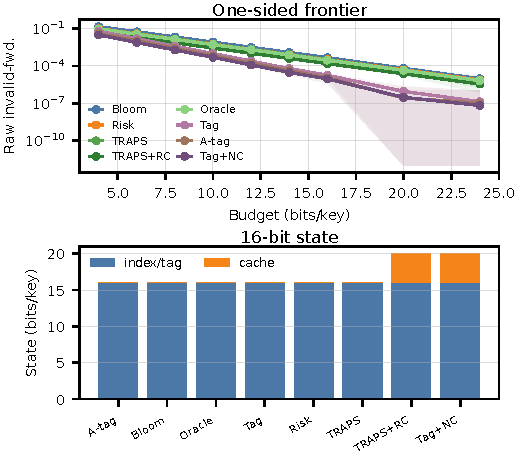
\includegraphics[width=\linewidth]{figure/icde_experiments/icde_frontier_production.pdf}
  \caption{Seeded admission-index frontier with production baselines.}
  \label{fig:icde-production-frontier}
\end{figure}

\subsection{Admission-Index Microbenchmarks}
\label{sec:exp-index-microbench}

\paragraph{Seeded production-baseline frontier}
Figure~\ref{fig:icde-production-frontier} compares admission-index baselines across 30 common-random-number seeds. Each seed uses 200k represented keys, 50k valid probes, and one million invalid probes; the reported data include raw and first-seen denominators, seed-level rates, 95\% intervals, and memory breakdowns. At 16 bits per represented key, Global Bloom forwards \(4.63\times10^{-4}\) of invalid probes on average. Handcrafted risk partitioning and TRAPS learned allocation reduce AMQ forwarding to \(3.21\times10^{-4}\) and \(3.06\times10^{-4}\), respectively; adding exact replay suppression lowers TRAPS's raw invalid-forward rate to \(1.55\times10^{-4}\) while preserving the same first-seen rate. The non-deployable oracle AMQ reaches \(2.90\times10^{-4}\), showing the remaining physical-design headroom.

Peppered fast tags give the exact-fingerprint frontier: observed uniform 16-bit tags forward \(1.78\times10^{-5}\), close to the \(2^{-16}\) calibration target, and adaptive account-risk tags forward \(1.09\times10^{-5}\). A production 64-bit tag bound is reported separately as a zero-event upper-bound row and is not plotted as part of the 16-bit frontier. The AMQ frontier answers a different physical-design question: given a one-sided approximate-membership frontend with residual false forwards, TRAPS allocates that residual channel across risk regions. The handcrafted risk row is a strong domain baseline with generator-aligned risk markers; the learned row tests automatic region discovery under the same capped AMQ allocation and replay machinery. Operational rate-limit-plus-tag hybrids reduce invalid forwards further but throttle valid requests, so they are reported separately from one-sided indexes.

\begin{figure}[t]
  \centering
  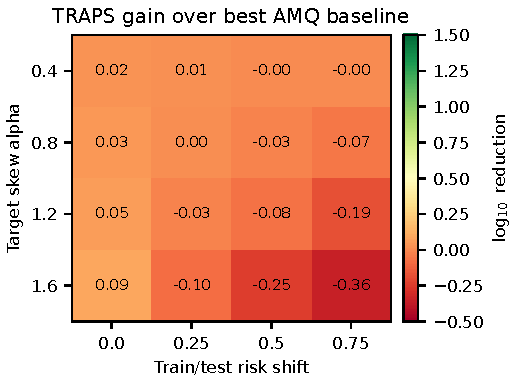
\includegraphics[width=\linewidth]{figure/icde_experiments/icde_shift_grid_heatmap.pdf}
  \caption{Distribution-shift grid. Cell values are median \(\log_{10}\) reduction of TRAPS over the best non-learned AMQ baseline; negative cells mark frozen-router degradation.}
  \label{fig:icde-shift-grid}
\end{figure}

\paragraph{Shift grid and worst cases}
Figure~\ref{fig:icde-shift-grid} sweeps target-account skew and train/test risk drift at 12 and 16 bits/key; separate exported sensitivity varies replay fraction and occupancy injection. TRAPS improves over non-learned AMQs when high-risk misses remain aligned with validation-time regions, and the grid also identifies when a frozen allocation should be refreshed. Table~\ref{tab:shift-dynamic} gives the 16-bit worst-case accounting: the worst frozen cell reaches \(1.51\times10^{-3}\), while previous-window next-epoch allocation and drift guard bring the worst case back near Global Bloom. Large drift is therefore a measured rebuild/fallback condition in the control plane.
The dynamic rows are the operational policy: frozen routing is the stale-state ablation, while next-epoch capacity and drift guard use only previous-window observations.

\begin{table}[t]
\centering
\caption{Shift/fallback accounting at 16 bits/key. Values are first-seen invalid-forward rates over 160 shift cells; dynamic rows use previous-window observations without future labels.}
\label{tab:shift-dynamic}
\scriptsize
\setlength{\tabcolsep}{3.3pt}
\begin{tabular}{lrrrr}
\toprule
Method & Median & P95 & Worst & Fallback cells \\
\midrule
Global Bloom & 4.59e-04 & 4.59e-04 & 4.59e-04 & 0 \\
Frozen TRAPS & 4.37e-04 & 1.00e-03 & 1.51e-03 & 0 \\
Dynamic next epoch & 3.76e-04 & 4.22e-04 & 4.36e-04 & 0 \\
Drift guard & 3.80e-04 & 4.58e-04 & 4.58e-04 & 20 \\
\bottomrule
\end{tabular}

\end{table}

\begin{figure*}[t]
  \centering
  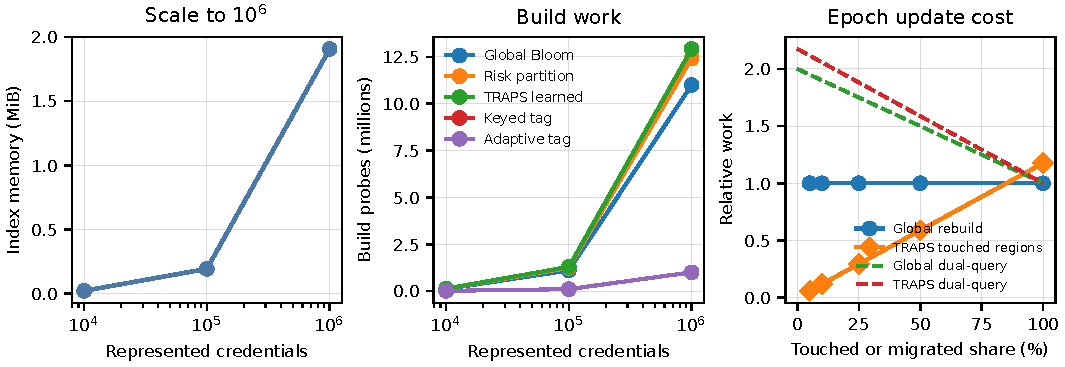
\includegraphics[width=\linewidth]{figure/icde_experiments/icde_scale_update_sweep.pdf}
  \caption{Scale and update behavior at 16 bits per represented credential.}
  \label{fig:icde-scale-update}
\end{figure*}

\paragraph{Scale and update cost}
Figure~\ref{fig:icde-scale-update} extends the index experiment to \(10^6\) represented credentials. At 16 bits per credential, the AMQ state is about 1.9 MiB for \(10^6\) entries before allocator metadata and replay-cache state. Build work scales linearly with represented credentials; the learned TRAPS allocation uses about 12.9 expected Bloom probes per invalid query at this budget, compared with 11 for a global Bloom filter and 1 for keyed tags. The update panel illustrates the operational value of regioning: routing-preserving updates that touch a subset of regions rebuild proportional state, while dual-query migration has a bounded transient probe multiplier that falls as credentials migrate.

\begin{figure*}[t]
  \centering
  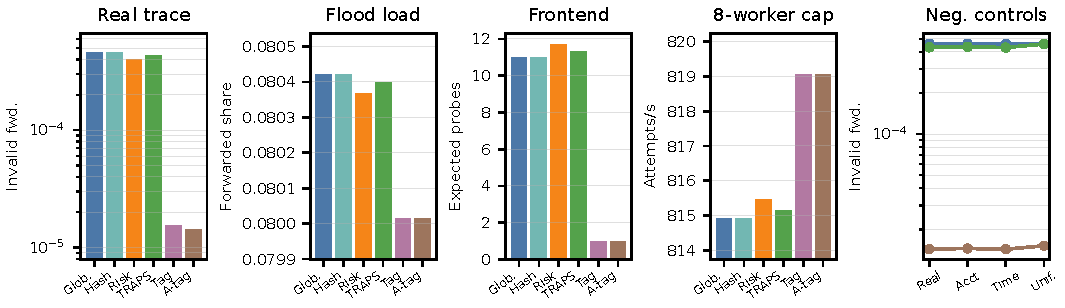
\includegraphics[width=\linewidth]{figure/icde_experiments/icde_lanl_trace_suite.pdf}
  \caption{LANL-conditioned routing/skew replay and router ablation.}
  \label{fig:icde-lanl-trace}
\end{figure*}

\subsection{Public Trace-Conditioned Replay}
\label{sec:exp-lanl}

\paragraph{LANL trace setup}
The public LANL authentication trace~\cite{Turcotte2018UnifiedHostNetwork} provides real enterprise arrival order, account/source skew, burstiness, routing-feature drift, and Success/Fail authentication status. The experiment samples 750{,}000 chronological events, uses the first 60\% for training, the next 20\% for validation, and the final 20\% for testing. The default full-stable token concatenates destination user, destination host, authentication type, logon type, and orientation. Source host, source user, status, and future fields are excluded from the token and router features. The exported denominator files report 8{,}702 destination users, 4{,}077 sources, top-1\% user event mass of 0.400, user-event Gini 0.753, and train/test token JS divergence 0.180.

\paragraph{Trace-conditioned baselines}
The LANL suite has two outcome views. First, a status-outcome replay uses the trace's real Success/Fail status as the event label. It yields 138{,}390 represented-success test events and 1{,}080 failure events; TRAPS learned routing forwards \(2.10\times10^{-7}\) of failures in expectation, versus \(4.59\times10^{-4}\) for Global Bloom and \(3.25\times10^{-4}\) for handcrafted risk partitioning, with zero represented-success false rejects. Second, an invalid-heavy stress replay uses the same LANL arrival/account/source skew with generated password-validity labels, yielding 7{,}015 represented-valid and 140{,}297 invalid test events. In that stress view, Global Bloom forwards \(4.59\times10^{-4}\), handcrafted risk partitioning \(3.98\times10^{-4}\), TRAPS learned routing \(4.32\times10^{-4}\), keyed tags \(1.53\times10^{-5}\), and adaptive tags \(1.44\times10^{-5}\). This split makes the trace result useful for both routing and substrate interpretation: the learned route extracts metadata signal in the status-outcome view, while the invalid-heavy view keeps a large denominator and shows exact tags as the fast-verifier frontier.

\paragraph{Learned-router ablation and sensitivity}
Account-shuffle, time-shuffle, and uniform-risk controls test whether routing uses enterprise metadata skew rather than future labels. Destroying risk information moves TRAPS back to the global Bloom rate. The status-outcome replay supplies real trace outcomes, while the invalid-heavy stress replay keeps the credential-flood denominator large enough to compare AMQ allocation policies.

\subsection{Named Workload Corners}
\label{sec:exp-corners}

The full grid carries the main evidence; the named KPwA/CPwA workloads provide interpretable corners. In the fixed-credential \emph{Credential-Flood Day} corner, TRAPS preserves the one-sided invariant and reduces invalid forwarding relative to the same-memory Global Bloom baseline when the learned regions match the attack skew. In the \emph{Occupancy-Injection Attack} corner, attacker-controlled insertions stress region capacity; the shift grid and ablation table expose the corresponding cap and refresh behavior across all cells.

\subsection{Ablation Study}
\label{sec:exp-ablation}

We next isolate learned partitioning, region-wise allocation, replay suppression, and capped allocation.

\begin{table}[t]
  \centering
  \scriptsize
  \caption{Mechanism ablation at 16 bits/key over 30 seeds.}
  \label{tab:traps-ablation}
  \begin{tabular}{lrrrr}
\toprule
Variant & Raw IFFR & First-seen IFFR & Backend calls & Cap viol. \\
\midrule
Full & 1.56e-04 & 3.12e-04 & 50156 & 0 \\
Hash router & 4.59e-04 & 4.59e-04 & 50452 & 0 \\
Equal alloc. & 4.59e-04 & 4.59e-04 & 50460 & 0 \\
No cap & 1.32e-04 & 2.65e-04 & 50136 & 2 \\
No replay & 3.12e-04 & 3.12e-04 & 50312 & 0 \\
Oracle & 1.48e-04 & 2.96e-04 & 50146 & 0 \\
\bottomrule
\end{tabular}

\end{table}

Table~\ref{tab:traps-ablation} separates raw invalid forwards from first-seen invalid forwards. Removing the learned router or region-wise allocation returns the AMQ close to the global Bloom rate. Removing replay suppression leaves the first-seen rate unchanged but doubles raw invalid forwards under a 50\% replay fraction, which is the expected behavior for an exact negative cache. The no-cap row can improve the median rate but creates cap violations, so it is not a safe deployment policy.

The main paper focuses on the ablation rows that directly test the ICDE claim: learned routing, allocation, replay suppression, and cap enforcement.

\begin{figure}[t]
  \centering
  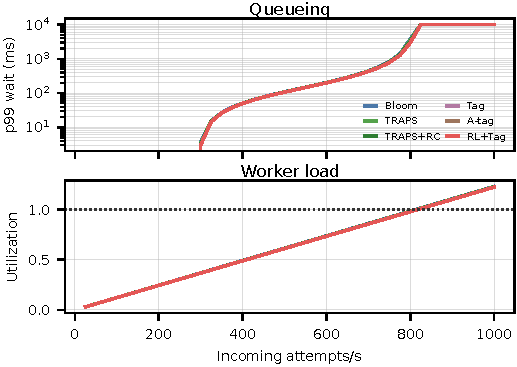
\includegraphics[width=\linewidth]{figure/icde_experiments/icde_queueing_by_method.pdf}
  \caption{Method-specific bounded-worker queueing with measured Argon2 service time.}
  \label{fig:icde-queueing}
\end{figure}

\subsection{Backend Saturation and Replay State}
\label{sec:exp-queueing-replay}

\paragraph{Bounded-worker queueing}
Figure~\ref{fig:icde-queueing} maps method-specific forwarding rates from the production frontier to backend-worker pressure using the 122.07 ms Argon2 mean service time and eight backend workers. With an 8\% valid-attempt fraction, all one-sided indexes keep utilization close because valid attempts dominate residual backend work; rate-limit hybrids are plotted with their measured valid-drop caveat rather than mixed into the one-sided frontier.
The queueing panel translates forwarding-rate deltas into worker provisioning and latency headroom under the shared backend service-time model.

\begin{figure}[t]
  \centering
  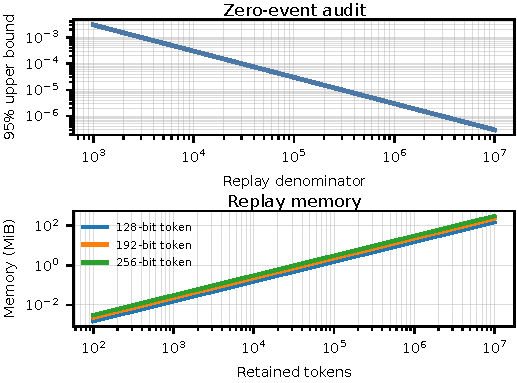
\includegraphics[width=\linewidth]{figure/icde_experiments/icde_replay_cache_ci.pdf}
  \caption{Replay-cache memory and finite zero-event audits.}
  \label{fig:icde-replay-cache}
\end{figure}

\paragraph{Replay cache and zero-event audits}
Figure~\ref{fig:icde-replay-cache} summarizes finite-audit and replay-state accounting. Zero events over \(10^5\) trials gives a 95\% upper bound of about \(3.0\times10^{-5}\), while retaining \(10^6\) backend-confirmed invalid tuples costs about 15.3 MiB with 128-bit tokens and 30.5 MiB with 256-bit tokens before hash-table overhead.

\subsection{Discussion and Limitations}
\label{sec:exp-limitations}

TRAPS reduces calibrated backend verification work while preserving zero observed pre-screening false rejects in the evaluated replays. The gains come from different layers: exact keyed tags define the strongest account-local fast-verifier frontier, while AMQ-backed TRAPS contributes capped residual-channel allocation, replay suppression, and migration-safe capacity control. The controlled generator keeps the KPwA and CPwA stress tests reproducible and varies attack skew, insertion pressure, and queueing load in isolation.

The end-to-end figures use a frozen epoch allocation selected from training and validation statistics. Section~\ref{sec:dynamic-capacity} specifies next-epoch capacity adjustment under changing KPwA mixtures, CPwA insertion pressure, and replay-cache discoveries; the scale/update experiment shows how rebuild and dual-query costs grow with represented credentials and touched regions.

The empirical adversary is the partial-information attacker from our threat model: it does not observe exact region assignments, thresholds, live filter state, or local drop decisions. With per-region caps, Section~\ref{sec:correctness-bound} bounds expected backend work per distinct invalid tuple by \(\varepsilon_{\mathrm{cap}}\), complementing robust-Bloom-filter notions~\cite{Naor2015AdversarialBF,NaorOved2022BetOrPass,LotanNaor2025MonotonicityBetting,Tirmazi2025PrivacyModelBF} with backend-work accounting and exact replay retention.

Production deployments integrate the admission index with concurrency control, queueing, latency padding, monitoring, abuse-response policy, and rebuild scheduling. The no-false-reject property relies on stable routing, atomic insertion, and versioned dual-query rebuilds; stale Bloom-filter bits from password changes are handled through periodic rebuilds or dynamic AMQ variants. TRAPS assumes a trusted first-party frontend, which matches the intended placement before the service's own password verifier.
